\documentclass{template/openetcs_article}

\usepackage{todonotes}
\usepackage{tikz}
\usepackage{style/tikz-uml}
\usepackage{xspace}
\usepackage{rotating,url,color}
\setcounter{tocdepth}{3}
\usepackage{graphicx}
%\usepackage{lmodern}
\usepackage{multirow}
%\usepackage[table]{xcolor}
\usepackage{datetime}

\urldef{\mailboth}\path|{huang,jp}@informatik.uni-bremen.de|
\newcommand{\keywords}[1]{\par\addvspace\baselineskip
\noindent {\bf Keywords} \enspace\ignorespaces#1}

\usetikzlibrary{arrows,positioning,fit,shapes,calc}


\newcommand{\ops}{\ensuremath{\operatorname{ops}}}
\newcommand{\ITE}{\ensuremath{\operatorname{ite}}}
\newcommand{\IF}{\ensuremath{\operatorname{if}}}
\newcommand{\THEN}{\ensuremath{\operatorname{then}}}
\newcommand{\ELSE}{\ensuremath{\operatorname{else}}}
\newcommand{\ENDIF}{\ensuremath{\operatorname{endif}}}
\newcommand{\TRUE}{\ensuremath{\operatorname{true}}}
\newcommand{\FALSE}{\ensuremath{\operatorname{false}}}

 \pgfarrowsdeclare{squarea}{squarea}%{{-.5bp}{8.5bp}}
 {
   \arrowsize=0.4pt
   \advance\arrowsize by.275\pgflinewidth%
   \pgfarrowsleftextend{+-.5\pgflinewidth}
   \advance\arrowsize by7\arrowsize
   \advance\arrowsize by.5\pgflinewidth
   \pgfarrowsrightextend{+\arrowsize}
 }
 {
   \arrowsize=0.4pt
   \advance\arrowsize by.275\pgflinewidth%
   \pgfsetdash{}{+0pt}
   \pgfsetroundjoin
   \pgfpathmoveto{\pgfqpoint{8\arrowsize}{4\arrowsize}}
   \pgfpathlineto{\pgfqpoint{0\arrowsize}{4\arrowsize}}
   \pgfpathlineto{\pgfqpoint{0\arrowsize}{-4\arrowsize}}
   \pgfpathlineto{\pgfqpoint{8\arrowsize}{-4\arrowsize}}
   \pgfpathclose
   \pgfusepathqstroke
 }
 
 \newtheorem{example}{Example}
 
 

 
  \tikzset{
  constraint/.style = {rounded corners, draw, align=center, inner sep=8pt},
  binding/.style = {->, >=squarea, shorten >= -4.5pt},
  double binding/.style = {<->, >=squarea, shorten >= -4.5pt, shorten <= -4.5pt},
  parameter/.style = {draw, align=center, inner sep=2pt}
  }
  \tikzset{
  initialstate/.style = {circle, fill=black},
  smstate/.style = {rounded corners, draw, align=center, inner sep=8pt},
  trans/.style = {->,thick}
  }

\renewcommand{\baselinestretch}{0.98}

\usepackage{hyperref}
\graphicspath{{./template/}{.}{./figures/}}

%\DeclareMathSymbol{\B}{\mathalpha}{AMSb}{"42}
\DeclareMathSymbol{\I}{\mathalpha}{AMSb}{"49}
\DeclareMathSymbol{\N}{\mathalpha}{AMSb}{"4E}
\DeclareMathSymbol{\Pwr}{\mathalpha}{AMSb}{"50}
\DeclareMathSymbol{\Q}{\mathalpha}{AMSb}{"51}
\DeclareMathSymbol{\R}{\mathalpha}{AMSb}{"52}
\DeclareMathSymbol{\Z}{\mathalpha}{AMSb}{"5A}
\DeclareMathSymbol{\Sol}{\mathalpha}{AMSb}{"53}

\newcommand{\obsv}[1]{{\cal O}(#1)}
\newcommand{\ctrl}[1]{{\cal C}(#1)}
\newcommand{\vdot}[1]{\stackrel{.}{#1}}
\newcommand{\power}{\mathbf{P}}

\newcommand{\HS}{{\mathcal H}}

\newcommand{\Interval}{\I}

\newcommand{\ist}{\mbox{{\tt true}}}
\newcommand{\isf}{\mbox{{\tt false}}}
\newcommand{\emptytrace}{\langle~\rangle}
\newcommand{\abegin}{\mathbf{begin}}
\newcommand{\aend}{\mathbf{end}}
\newcommand{\alet}{\mathbf{let}}
\newcommand{\aendlet}{\mathbf{endlet}}
\newcommand{\ain}{\mathbf{in}}
\newcommand{\afor}{\mathbf{for}}
\newcommand{\adownto}{\mathbf{downto}}
\newcommand{\aforall}{\mathbf{foreach}}
\newcommand{\awhile}{\mathbf{while}}
\newcommand{\ado}{\mathbf{do}}
\newcommand{\aenddo}{\mathbf{enddo}}
\newcommand{\acontinue}{\mathbf{continue}}
\newcommand{\aif}{\mathbf{if}}
\newcommand{\athen}{\mathbf{then}}
\newcommand{\aelse}{\mathbf{else}}
\newcommand{\aelseif}{\mathbf{elseif}}
\newcommand{\aendif}{\mathbf{endif}}
\newcommand{\ainout}{\mathbf{inout}}
\newcommand{\aout}{\mathbf{out}}
\newcommand{\aprocedure}{\mathbf{procedure}}
\newcommand{\afunction}{\mathbf{function}}
\newcommand{\abreak}{\mathbf{break}}
\newcommand{\awhere}{\mathbf{where}}
\newcommand{\Sup}[1]{\overline{#1}}
\newcommand{\Inf}[1]{\underline{#1}}

\newcommand{\trl}{/\!/}



\newcommand{\taba}{\hspace*{3mm}{}}
\newcommand{\tabb}{\hspace*{6mm}{}}
\newcommand{\tabc}{\hspace*{9mm}{}}
\newcommand{\tabd}{\hspace*{12mm}{}}
\newcommand{\tabe}{\hspace*{15mm}{}}
\newcommand{\tabf}{\hspace*{18mm}{}}
\newcommand{\tabg}{\hspace*{21mm}{}}
\newcommand{\tabh}{\hspace*{24mm}{}}
\newcommand{\tabi}{\hspace*{27mm}{}}
\newcommand{\tabj}{\hspace*{30mm}{}}
\newcommand{\tabk}{\hspace*{33mm}{}}
\newcommand{\tabl}{\hspace*{68mm}{}}

             
                   
\newcommand{\gca}[1]{F(#1)}
\newcommand{\gcb}[1]{F^*(#1)}
\newcommand{\gclr}{{{L^*\atop\longleftarrow}\atop
                   {\longrightarrow\atop L}}}
\newcommand{\gclrf}{{{F^*\atop\longleftarrow}\atop
                   {\longrightarrow\atop F}}}                   
                   
\newcommand{\gclrj}{{{J^*\atop\longleftarrow}\atop
                   {\longrightarrow\atop J}}}
                                      
\newcommand{\gcaprime}[1]{F'(#1)}
\newcommand{\gcbprime}[1]{F'^*(#1)}
\newcommand{\gclrprime}{{{L'^*\atop\longleftarrow}\atop
                   {\longrightarrow\atop L'}}}  
                   
\newcommand{\gcaone}[1]{G(#1)}
\newcommand{\gcbone}[1]{G*(#1)}
\newcommand{\gclrone}{{{G^*\atop\longleftarrow}\atop
                   {\longrightarrow\atop G}}}                                    
                   
                                                         

\newcommand{\dontshow}[1]{}


\newcommand{\Nat}{{\mathbb N}}
\newcommand{\Real}{{\mathbb R}}

\newcommand{\trans}{\longrightarrow}
\newcommand{\transp}{\longrightarrow_{\power}}
\newcommand{\transl}{\longrightarrow_{L}}
\newcommand{\transg}{\longrightarrow_{G}}
\newcommand{\transcfg}[1]{\stackrel{#1}{\longrightarrow}_{CFG}}
\newcommand{\isdefd}{=_{\mbox{\footnotesize def}}}
\newcommand{\equivdef}{\equiv_{\mbox{\footnotesize def}}}
\newcommand{\mitem}{\mbox{\em M-Item}}
\newcommand{\fun}{\rightarrow}
\newcommand{\pfun}{\not\rightarrow}
\newcommand{\currt}{\hat{t}}

\newcommand{\dom}{\mbox{dom}}
\newcommand{\ran}{\text{ran}}

\newcommand{\sigmaa}{\sigma_A}
\newcommand{\strictimplies}{\stackrel{\bullet}{\Rightarrow}}

\newcommand{\eqc}[2]{[#1;#2]}

\newcommand{\vest}{{V_{\text{\sl est}}}}
\newcommand{\vmax}{{V_{\text{\sl MRSP}}}}
\newcommand{\wout}{\mathsf{W}}
\newcommand{\eout}{\mathsf{EB}}
\newcommand{\areb}{\text{allowRevokeEB}}
\newcommand{\sbia}{\text{SBAvailable}}
\newcommand{\sbz}{\text{sb}_0}
\newcommand{\ticmd}{\text{TICmd}}
\newcommand{\dmicmd}{\text{DMICmd}}

\newcommand{\sob}{\text{speedOnBoard}}
\newcommand{\std}{\text{speedToDriver}}
\newcommand{\pstd}{\text{permittedSpeedToDriver}}
\newcommand{\csmsw}{\text{csmSwitch}}
\newcommand{\sbicmd}{\text{sbiCmd}}
\newcommand{\sbidisplay}{\text{DMIdisplaySBI}}


\newcommand{\dvw}{\text{dV}_{\mathsf{warning}}}
\newcommand{\dvs}{\text{dV}_{\mathsf{sbi}}}
\newcommand{\dve}{\text{dV}_{\mathsf{ebi}}}

\newcommand{\calcw}{\text{dV\_warning(float)}}
\newcommand{\calcs}{\text{dV\_sbi(float)}}
\newcommand{\calce}{\text{dV\_ebi(float)}}
\newcommand{\calcstd}{\text{calc\_speed\_to\_driver()}}
\newcommand{\calcpstd}{\text{calc\_permitted\_speed\_to\_driver()}}
\newcommand{\calcsob}{\text{calc\_speed\_onboard()}}





\newcommand{\qpsc}{\text{qpsc}}
\newcommand{\inpunc}{\text{Input}_{\text{\sl unchanged}}}
\newcommand{\tpsc}{\text{tpsc}}
%\newcommand{\inpch}{\text{Input}_{\text{\sl changed}}}
%\newcommand{\outpun}{\text{Output}_{\text{\sl unchanged}}}


\newcommand{\ta}{\mathbf{A}}
\newcommand{\te}{\mathbf{E}}
\newcommand{\tx}{\mathbf{X}}
\newcommand{\tf}{\mathbf{F}}
\newcommand{\tg}{\mathbf{G}}
\newcommand{\tu}{\mathbf{U}}
\newcommand{\tr}{\mathbf{R}}
\newcommand{\tw}{\mathbf{W}}
\newcommand{\tgt}{\mathbf{G_{\text{\tiny T}}}}

%%%???\newcommand{\ts}{\mathbf{S}}
\newcommand{\ttt}{\mathbf{T}}
\newcommand{\ty}{\mathbf{Y}}
\newcommand{\tz}{\mathbf{Z}}
\newcommand{\too}{\mathbf{O}}

\newcommand{\xbox}{\unskip\nobreak\hfil\penalty50
      \hskip2em\hbox{}\nobreak\hfil$\Box$%
      \parfillskip=0pt \finalhyphendemerits=0 \par}



\begin{document}

% ===================================================================================
\frontmatter
\project{openETCS}
%============================
% The document metadata is defined below

%assign a report number here
\reportnum{OETCS/WP4/CSM~--~01/00}

%define your workpackage here
\wp{Work Package 4: ``Verification
\& Validation Strategy''\\
Work Package 7: Tool Chain}


%set a title here
\title{Combination of Behavioral and Parametric Diagrams for Model-based Testing --\\
Application to ETCS Target Speed Monitoring}

%set a subtitle here
\subtitle{Technical report}

%set the date of the report here
\date{2015-11-25}

% define the coverart
\coverart[width=350pt]{openETCS_EUPL.png}
 
%define the type of report
\reporttype{Technical Report}

\author{Felix H{\"u}bner \and  Christoph Hilken \and Jan Peleska}
\affiliation{University of Bremen}


\begin{abstract}
This technical report contributes to the openETCS project, work packages 
WP4 -- Verification \& Validation Strategy, and WP7 -- Tool Chain. 
The technology presented here allows for the incorporation of braking curves and 
other time-continuous behaviours of trains into test models, from where test cases, 
concrete test data, and test procedures can be automatically generated.
The proposed technology is currently implemented in the RT-Tester tool which has been 
made available for the openETCS project as part of WP7.

Model-based testing is a promising approach to cope with the complexity 
of today's train control  systems. 
It shifts the effort from manual test case specification to the 
modeling of the system's behavior and enables automated test case generation.   
System behavior is often modeled by state machines. However, state machines are not 
appropriate to model all kinds of behavior, in particular time-continuous evolutions
such as time-dependent position, speed,  and 
acceleration of trains. This work combines state machines
and parametric diagrams of the Systems Modeling Language (SysML) to 
enable the description of time-discrete and time-continuous control in test models,
at the same time introducing a new concept for a higher degree of abstraction. This is shown by application 
to a real-word example: a safety function of the European Train Control System (ETCS), the so-called target speed monitoring function.


\keywords{Model-based testing, Equivalence class partition testing, UML/SysML, European Train Control System ETCS, Ceiling Speed Monitoring}
\end{abstract}

\maketitle

\section{Introduction}\label{sec:intro}
% ==========================================================================

\subsection{A Test Model for the ETCS Ceiling Speed Monitor}
In 2011 the {\it model-based testing benchmarks website} www.mbt-benchmarks.org has been 
created with the objective to publish test models that may serve as challenges or benchmarks 
for validating testing theories   and for comparing the capabilities of model-based testing (MBT) tools~\cite{pel2011a}.
In this technical report a novel contribution to this website is presented, a SysML model
of the Ceiling Speed Monitor (CSM) which is part of the European Vital Computer (EVC), the onboard controller of trains conforming to the European Train Control System (ETCS) standard~\cite{ETCS}. In    Section~\ref{sec:ceil} the functional objectives for the CSM are described, and in Section~\ref{sec:modeldesc} the detailed model description is provided. 

The static and behavioural semantics of SysML models have been defined in~\cite{SysML12,uml_2_4} in a semi-formal way, leaving certain ``semantic variation points'' open, so that they can be adjusted according to project-specific requirements. For automated model-based testing, however, a strictly formal semantics is required, so that concrete test data can be calculated from the model's transition relation using constraint solving techniques~\cite{peleska2013ictss}. 
We therefore describe in Section~\ref{sec:transrel} how a formal behavioural semantics is derived for the CSM model and present the associated transition relation in propositional form.

We use state transition systems (STS) for encoding the operational semantics of concrete
modelling formalisms like SysML. STS are widely known from the field of model checking~\cite{clarke_em-etal:1999a}, because their extension into Kripke Structures allows for effective data abstraction techniques. The latter are also applied for equivalence class testing. 
Since state transition systems are a means for semantic representation, testing theories elaborated for STS are applicable for all concrete formalisms whose behavioural semantics can be expressed by STS. In~\cite{d341} it is shown how the semantics of general SysML models and models of a process algebra are encoded as STS. In this technical report we illustrate  how this is achieved for the concrete case of the CSM SysML model.

% ==========================================================================
\subsection{Equivalence Class Partition Testing for the CSM}

The CSM represents a specific test-related challenge: its behaviour depends on actual and allowed speed, and these have conceptually real-valued data domains, so that -- even when   discretising
the input space -- it would be infeasible to exercise all possible combinations of 
inputs on the system under test (SUT). Therefore equivalence class partition (ECP)
 testing strategies have 
to be applied for testing the CSM. While these strategies are well-adopted  in a heuristic manner
in today's industrial test campaigns, practical application of equivalence class testing still lacks 
formal justification of the equivalence classes selected and the sequences of class representatives 
selected as test cases: standard text books used in industry, for example~\cite{spillner2006}, 
only explain the generation of input equivalence class tests for   systems, where the 
SUT reaction to an input class representative is independent on the internal state. Moreover, the systematic calculation of classes from models, as well as their formal justification with respect to
test strength and coverage achieved, is not yet part of today's best practices in industry. 

In contrast to this, formal approaches to equivalence class testing have been studied in the formal methods communities; references to these results  are given in Section~\ref{sec:related}.
In the second main part of this report (Section~\ref{sec:iecpstart}) we therefore describe a recent formal technique for equivalence class testing and its application to testing the CSM. The theoretical 
foundations of this strategy have been published by two of the authors in~\cite{peleska2013ictss}. 
This technical report illustrates its practical application and presents first evaluation details using a 
prototype implementation in an existing MBT tool; the ECP tests are  compared to test results obtained when applying other MBT coverage strategies, such as transition cover or MC/DC coverage (Section~\ref{sec:conventionaltests}). 


% ==========================================================================
\subsection{Fault Models and Completeness Results}


Our ECP strategy
introduces test suites depending on {\it fault models}. This well adopted notion has first been 
introduced in the field of finite state machine (FSM) testing~\cite{petrenko1996}, but is also applicable
to other formal modelling techniques. A fault model consists of a reference model, a conformance relation and a fault domain. The latter is a collection of models whose behaviour may or may not be
consistent to the reference model in the sense of the conformance relation. The test suites generated 
by the ECP strategy described here are {\it complete} with respect to the given fault model: each
system of the fault domain which conforms to the reference model will pass all the generated tests
(this means that the test suite is {\it sound}), and each system in the fault domain that violates the
conformity to the reference model will fail at least  once when tested according to the test suite (the test suite is {\it exhaustive}). 




%%% @todo open proof strategy of the openETCS project





\section{Background}
In order to keep this paper self contained relevant parts of the European Train Control System and the Systems Modeling Language are introduced. 
\subsection{European Train Control System}
The European Train Control System (ETCS) shall replace existing national train control systems by a modern unified
 system in the European Union. The system
requirement specification is publicly available~\cite{ETCSSRS-Principles}. 

The onboard computer of ETCS trains (the so-called \emph{European Vital Computer
(EVC)}) performs -- among other safe\-ty-relevant control tasks -- \emph{target
speed monitoring (TSM)}: the speed of the train, while approaching a target (for
example, a train station or a level crossing), is monitored by the EVC, so that
the ability to brake the train in time for the target is always
ensured~\cite{ETCSSRS-Principles}. To this end, the speed-dependent
\emph{braking curves} of the train have to be taken into account, so that the
braking distance required is correctly calculated.

% As part of the ETCS, the onboard computer of the train (European
% Vital Computer, EVC) shall supervise the train. One safety function of the EVC
% is the train's speed and distance monitoring. This safety function supervises and enforces speed and distance limits. 
% The function can operate in three exclusive modes. One of them is the ``Target
% Speed Monitoring'' (TSM).
% This mode is active if a train approaches a target location (train station,
% signal,\ldots). In this mode the train's current speed $V_\text{est}$ is
% supervised according to the
% maximum allowed speed ($V_\text{mrsp}$) and the distance to a target location, where
% the train shall stop. Usually this location is in front of a signal. This TSM function 
% shall serve as a running example, to illustrate our approach and to give a proof
% of concept by application to a complex real world example.

In the remainder, the following variables are used: $v_\text{est}$ is a system input describing the 
current train speed. The maximum allowed speed on the track section of the train is denoted by $v_\text{mrsp}$. The value
of $v_\text{mrsp}$ should remain constant over time, while $v_\text{est}$ should change according to the current
acceleration $a$.  
All track related locations, including the train position, are measured as track relative distances $D$,
starting from zero (start location) and ending at the target location $D_\text{Target}$.
The train position is given by variable $D_\text{front}$ and should always have
values from the range $[0,D_\text{Target}]$. $D_\text{Target}$ is constant during runtime, while $D_\text{front}$ might change
over time as the train moves forward towards the target location. 

\subsection{Systems modeling language}

OMG's \emph{Systems Modeling Language SysML}~\cite{SysML15} is a semi-formal language to specify a model of the system's structure and behavior. In addition, corresponding diagrams offer a graphical representation of parts of the model. Therefore, a system description is composed of different kinds of diagrams, for example block definition diagrams and internal block diagrams to describe the structure, complemented by activity and state machine diagrams to describe the behavior of the system. Our approach is working on state machines and constraint blocks. Therefore, to focus on the objectives of this paper, in the remainder only parametric diagrams and state machine diagrams are used. 



\paragraph{Constraint blocks}
Constraint blocks are used to
express general dependencies between observables, such as physical laws. 
Parametric diagrams are used to bind the generic names of these observables to the
concrete model variables that are restricted by these constraints. Using these syntactic
entities, the boundary conditions restricting time-continuous inputs or outputs of  
the SUT can be suitably specified. 

\begin{example}
For the TSM function the braking distance has to be calculated. The motion of a train can be expressed by the
equations for a translational acceleration, which are $v=a t + v_o$ and
$s=\frac{1}{2} a t^2 + v_0t + s_0$. In Figure~\ref{fig:brakingdistance} both
expressions are combined to calculate the braking distance $s$. The constraints are bound 
to the system inputs ($v_\text{est}$ and $a$) in the parametric diagram.
\end{example}
SysML does not define a language to express constraints. In the remainder the natural mathematical notation is used, which is interpreted by our tools. In addition, it is possible to add conditions under which constraints are valid. Therefore, pseudocode is used. 
In particular, such conditioned constraints can be used to specify the
so-called \emph{flow conditions} of \emph{hybrid automata} associated with control modes specified in 
state machines: following~\cite{Hen96}, these flow conditions describe the 
restrictions to be observed by time-continuous variables, while the system resides in the
given control mode. 
\begin{figure}
\centering
\begin{tikzpicture}
\node[constraint] (c1) {Braking Time\\$\{0=a_b t_b + v_0\}$};
\node[constraint,below=1cm of c1] (c2) {Braking Distance\\$\{s=\frac{1}{2}a_b t_b^2 + v_0 t_b\}$};
\node[parameter, left=2cm of {$(c1)!0.5!(c2)$}] (p1) {$v_\text{est}$};
\node[parameter, right=2cm of {$(c1)!0.5!(c2)$}] (p2) {$a$};
\node[parameter, below=of c2] (p3) {$s$};
%\node[constraint,below=1cm of c2] (c3) {Safe Distance\\$\{d_{\text{safe}}=d_{\text{target}}-s\}$};
\draw[double binding] (c1) -- node[right, very near end]{$t_b$} node[left, very near start]{$t_b$} (c2);
\draw[binding] (p1) |- node[above, near end] {$v_0$}(c1);
\draw[binding] (p2) |- node[above, near end] {$a_b$}(c1);
\draw[binding] (p1) |- node[below, near end] {$v_0$}(c2);
\draw[binding] (p2) |- node[below, near end] {$a_b$}(c2);
\draw[binding] (p3) -- node[right, very near end] {$s$} (c2);
\end{tikzpicture}
\caption{Parametric diagram for the calculation of the braking distance}
\label{fig:brakingdistance}
\end{figure}


\paragraph{State machines and testing strategies}
UML's state machines have been adopted for SysML without changes. Hence, SysML state machines are
a variant of Harel's~statechart~formalism~\cite{harel96}. Therefore, many
MBT-tools are using state machines as modeling
formalism,~e.g.\cite{ali_searchbased_2011, bouquet_subset_2007} and many testing
strategies have been developed in respect to state machines. This includes
conventional strategies based on coverage criteria, but also complete test
strategies, that give a guarantee that certain types of faults are revealed,
given an assumption that only pre-defined types of faults can occur. In
addition, it was shown in~\cite{hubner_experimental_2015} that test suites
generated by a complete test strategy can have a very high test strength even if
the assumption for completeness does not hold.


\section{Problem Formulation and\\ General Idea}
As mentioned before, state machines have been shown suitable to model the behavior of reactive systems in the past and MBT approaches chose them as description means for their input models. With respect to upcoming cyberphysical-systems state machines are not convenient, especially, due to the integration of components, such as sensors and actuators in today's embedded systems. Such hybrid systems can be described by a combination of state machines and conditioned constraint blocks. 
Constraint blocks and parametric diagrams are well suited to describe mathematical expressions, as for example physical laws, due to their declarative manner. State machines on the opposite are an imperative, state-based description means and, hence, are not convenient to specify physical properties of the system. 
There are many approaches in the field of control theory and simulation to handle physical properties, but in the field of MBT physical constraints are usually neglected or simplified and current test strategies do not take them into account. As a consequence, test cases generated using current tools and strategies may be unrealistic and violate physical constraints. 

\begin{example}
Assume test cases shall be generated for the TSM function. Without considering
physical laws, a concrete test case might be generated that contains a
sequence of train speed values that have sudden jumps from very low to very high
values.
Such a behavior is unrealistic, since the acceleration of a train is bounded by
the train engine and train brakes.
Figure~\ref{fig:temporal-evolution} describes the physical constraints, that
model how the speed and position of a train should evolve over time. Considering
this kind of physical constraints leads to test cases that are executable in a
real environment.
\end{example}

To overcome this situation and to allow the utilization of parametric diagrams as well as constraint blocks, we propose the following approach:\\
%\begin{tikzpicture}
%\node[draw,align=left] (sm) {State\\ Machine};
%\node[draw,align=left,right=1.5cm of sm] (at) {Abstract\\ Test\\ Cases};
%\node[draw,align=left,right=1.5cm of at] (ct) {Concrete\\Test\\Cases};
%\node[draw,align=left,above= of {$(at)!0.5!(ct)$}] (param) {Parametric\\Diagram}; 
%\draw[thick,->] (sm)-- node[above=0.5cm,pos=0.5] (ecpt){ECPT} node[below,pos=0.5] {Step 1} (at);
%\draw[thick,->] (at)-- node[below,pos=0.5] {Step 2} (ct);
%\draw[thick,->] (param) |- (ct);
%\end{tikzpicture}\\ 
In a first step using an abstracted version of the state machine, abstract test cases are generated. 
Such an abstracted version is a so-called \emph{simulation} of the concrete system~\cite{clarke_em-etal:1999a}; the former represents an over-approximation of the latter. The simulation can easily be obtained by using Boolean variables as guard condition for every transition in the state machine. These Boolean variables are not restricted on the state machine level but bound to concrete system variables in the parametric diagrams.\footnote{
Given a concrete system description by means of a state machine, this simulation can as well be obtained automatically. 
But in most cases, the a priori modeling of an abstract state machine description of the system might be more natural and reduce the modeling
effort, as will be shown in section~\ref{sec:evaluation}.}
%The simulation is obtained by abstracting guard conditions to Boolean variables, if needed. 
Abstract test cases are constructed from this simulation model using an
input equivalence class partitioning 
test strategy with proven error detection capabilities~\cite{huang_complete_2014}. \footnote{Apart from that, the proposed approach allows the application of every other state machine based testing strategy}
The  inputs associated with an abstract test case are sequences of input equivalence classes.

In the second step, the abstract input sequences are resolved to sequences of concrete
model variable valuations, using a mathematical constraint solver. 
For this step,   the bindings of abstract Boolean
condition variables to concrete model variables defined by parametric diagrams are taken into account.
Additional physical constraints describing the temporal evolution  of system variables are considered
in this step as well, which leads to realistic concrete test cases. 

\begin{figure}
\centering
\begin{tikzpicture}
\node[constraint] (c1) {$\frac{d v}{d t}=a$};
\node[constraint, below=of c1] (c2) { $ -10 \leq a \leq 2$ };
\node[constraint, right=2 of c1] (c3) {$\frac{d D}{d t}=a*t+v$};
\node[align=left,constraint, below=of c3] (c4) {$a\leq A_\text{s}$ \\ $\IF$ TSM.inState(EB)};

\node[parameter, left=1.2cm of c1,above=0.6cm of c3] (df) {$D_\text{front}$};
\node[parameter, above right=0.2cm and 0.5cm of c1] (ve) {$v_\text{est}$};
\node[parameter, above left=0.2cm and 0.3cm of c4] (As) {$A_\text{safe}$};

\draw[binding] (df) -- node[above,right] {$D$} (c3);
\draw[binding] (ve) -| node[near end, left] {$v$} (c1.50);
\draw[binding] (ve) -| node[near end, left] {$v$}(c3.150);
\draw[binding] (As) -| node [near end, left] {$A_\text{s}$} (c4.150);

\draw[double binding] (c1) -- node[right,near start] {$a$} node [near end, right] {$a$} (c2);
\draw[double binding] (c1) -- node[near start, above] {$a$} node [near end, below] {$a $}  (c3);
\draw[double binding] (c3) -- node[near start, right] {$a$} node [near end, left] {$a$} (c4);
\end{tikzpicture}
\caption{Parametric diagram describing the temporal evolution of the TSM}
\label{fig:temporal-evolution}
\end{figure}


\section{Two-step Approach}




% Two-step approach:
% first step: over-approximation, build a statemachine with input equivalence
% classes. 
% 
% 
% In the current flow of the ECPT\todo[inline]{ECPT erklaeren in Background}
% approach tests are generated automatically from the state machine. At first the state machine is transformed into an internal
% representation. The behavioral semantics are defined by a state transition
% system. On this an input equivalence class partitioning is applied, resulting in
% a finite state machine, on which the W-method can be applied. By selecting
% concrete test data from the input equivalence classes, concrete test cases can
% be obtained. Concrete test data can be calculated, because all concrete system
% inputs state changes are modeled explicitly by state machines. 
% 
% Drawbacks: no notion of time, modelling effort


\paragraph{Step~1. System abstraction}

In the first step, the system behavior is abstracted. The idea is to use an 
overapproximation of the specified system's behavior: all traces possible in the concrete system based on the specification, considering all
physical and system related constraints, are also observable in the abstract
model. Whether a trace in the abstract model has a concrete solution in the real
world, depends on the abstraction and constraints. This is a conservative
approach, which guarantees that every system behavior is covered by the model,
while unrealistic traces might remain. If in the second step, no concrete
solution for an abstract test exists, it can be deduced, that this behavior is
not possible (assuming that the constraints are correct), and therefore it is
safe to neglect this test case.

%In the model abstraction, guard conditions occurring in state machines are 
%abstracted by Boolean variables, following the technique for generating simulations
%as described in~\cite{clarke_em-etal:1999a}. Additional physical constraints modeled in 
%constraint blocks are disregarded at this stage. Every state sequence that may occur
%in the concrete system is represented by an   


\begin{example}
\label{ex:abstraction}
%One way to include abstraction is to introduce abstract input symbols.
Consider  the following complex boolean expression, taken from the
ETCS specification \cite{ETCSSRS-Principles}:

\begin{align}
V_\text{est} > V_\text{mrsp} + DV_\text{ebi}(V_\text{mrsp}) 
\lor D_\text{front} > D_\text{EBI} 
\end{align} 

This boolean expression describes a trigger condition for the onboard controller
of the train to automatically activate the 
%If the condition is fulfilled, the system shall automatically activate the
%train's 
emergency brakes. Variable $V_\text{est}$ describes the current train
speed.
If this speed exceeds the maximum allowed speed $V_\text{mrsp}$ by more than an
offset $DV_\text{ebi}$, the emergency brakes are activated. Alternatively,
%If the train speed is
%below this threshold, but 
if the front of the train $D_\text{front}$ is too close
to the target location (this is expressed by $D_\text{front} > D_\text{EBI}$), the emergency brakes are
activated as well.

Instead of explicitly describing this trigger condition by concrete model variables, an abstract input variable
$t_{13}$ is introduced. The state machine transition that uses this abstract input variable looks like
this:
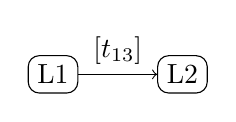
\begin{tikzpicture}
\node[draw,rounded corners] (l1) {L1};
\node[draw,rounded corners, right=1cm of l1] (l2) {L2};
\draw[->] (l1) -- (l2) node[pos=0.5,above] {$\lbrack t_{13}\rbrack$};
\end{tikzpicture}.
In this case we introduced a new free input variable. It can be assumed, that
the value of this variable can change arbitrarily over time. This is a safe
overapproximation of the real system.
\end{example}

The replacement of a complex guard-condition by a new boolean input
variable is always possible, but $n$ replacements introduce $n$ new inputs.
In the worst case this results in $2^n$ new input equivalence classes of the SUT~\cite{huang_complete_2014}: each feasible conjunction of the positive or negated 
Boolean expressions associated with each of the abstraction variables $t_i$ specifies
an input equivalence class.
For realistic models, 
not all combinations of valuations of the complex conditions are possible.
Using an SMT solver, impossible input combinations can be dropped a priori. These combinations
are ignored in the test generation.  

With this abstract description of the system behavior at hand, we are able to
apply the test generation strategy 
presented in~\cite{huang_complete_2014} and create a test suite,
whose inputs are represented by abstract equivalence classes.
%Note that our approach described in this paper is independent of the concrete
%test strategy, and every other strategy could be applied as well.

\begin{example}
For our running example, the TSM function, we introduced nine abstract input variables. 
From the $2^9=512$ possible combinations, only eight combinations were valid. Two of the combinations
can be considered as equivalent~\cite{huang_complete_2014}. Thus, seven input equivalence classes
were calculated from our abstract model.
\end{example} 

The result of the first step in our test case generation is a set of
abstract test cases. An abstract test case is a sequence of system states
$\langle\bar{s}_0,\ldots,\bar{s}_n\rangle$, where $\bar{s}_i: V_\text{abstract} \rightarrow D$ is the
valuation function, mapping the (abstract) Boolean system variables $t_k$
 to their values $\bar{s}_i(t_k)$    in the
$i$-th state.

% ===============================================================
\paragraph{Step 2. Concretization}\label{sec:concretization}

While the first step defined abstract test cases that are related to
computations in the abstract test model, the second step
aims at constructing concrete test data.
%for system tests concrete test data is
%needed. For testing it is necessary to specify concrete test data composed
%of inputs that stimulate the SUT and outputs that can be observed.

A concrete test case is a sequence of concrete 
system states $\langle s_0,\ldots,s_n\rangle$. Each $s_i$ is a valuation function   
$s_i: V\cup  V_\text{abstract} \rightarrow D$,
where the concrete system variables $v$, including the inputs and outputs, as well as the 
abstraction variable introduced before, are mapped
to concrete values  $s_i(v)\in D$.

For the concretization of the test cases, parametric diagrams were
added as an additional description means. The 
abstract variables introduced in Step~1 have to be related to concrete system
variables by parametric diagrams.
Two types of constraints can be
defined: \emph{state invariants} and \emph{temporal evolution}.

State invariants constrain the concrete system variables in every state and, therefore, in every test step of the test case, these
invariants have to be fulfilled. In a parametric diagram
a state invariant can be described by a constraint property. A parametric
diagram with $m$ constraint properties that define state invariants
($\text{INV}_1,\ldots,\text{INV}_m$) yields the invariant:

$\text{INV} \equiv \bigwedge_{j=1}^{m} \text{INV}_j$

Invariants in the concrete system are also used 
to bind the values of abstract system variables to
the concrete guard conditions they are abstracting.
\begin{example}
Considering trigger condition $t_{13}$ from example~\ref{ex:abstraction} the corresponding parametric diagram is shown in Figure~\ref{fig:parametric}. In this diagram $t_{13}$ gets bound to its concrete guard condition. 
\end{example}
Given this invariant, and given an abstract test case
\mbox{$\langle\bar{s}_0,\ldots,\bar{s}_n\rangle$}, we want to calculate a concrete test case
\mbox{$\langle s_0,\ldots,s_n\rangle$} that uses the same valuations of the abstract 
system variables -- that is, the same equivalence classes -- as prescribed by the
abstract test case. This is encoded by the following formula, where
%
%
%
%. To describe this problem as an SMT instance, let
%$V_i$ denote the variable symbols from $V\cup V_\text{abstract}$ in the $i$-th state. $v_i$ denotes the variable $v$ in the
%$i$-th state. 
%In the following formulas, 
$\phi[t/x]$ denotes  the formula derived from $\phi$ by exchanging every free occurrence of $x$ by the term $t$.


\begin{align}
\bigwedge_{i=0}^{n}& \big(\bigwedge_{t\in V_\text{abstract}} s_i(t) =\bar{s}_i(t) \wedge {}\\
& 
%\text{INV}[\bar{s}_i(v')/v'\in V_\text{abstract},v_i/v\in (V\setminus V_\text{abstract})]
\ \ \text{INV}[s_i(v)/v, v\in V\cup V_\text{abstract}]\big)
\end{align}
The above formula can be solved by an SMT solver.
The result is a concrete mapping of variables from $V$ to concrete values.
Using these concrete values, a concrete test case $\langle s_0,\ldots,s_n\rangle$ is
calculated.
% 
%  \todo[inline]{ohne Gewaehr:
% was die folgende Formel ausdruecken soll:
% konkreter Testfall ergibt sich, indem man (a) die Werte aus dem abstrakten
% Testfall uebernimmt (b) fuer jedes i die Invarianten loesen laesst, um die
% konkreten Werte zu bekommen }
% $<s_0,\ldots,s_n>$ is a concrete test case of $<\bar{s}_0,\ldots,\bar{s}_n>$ if and only if 
% $\bigwedge_{i=0}^{n}(s_i|_{V\cap V_\text{abstract}}= \bar{s}_i|_{V\cap V_\text{abstract}} \land\text{INV}[x/s_i(x),y/\bar{s}_i(y)])$. 

Apart from that, the temporal evolution of system variables is described by means of parametric diagrams. 
In contrast to an invariant, such constraints describe the change of values between two test steps. For example it may necessary to constrain the change of velocity
and location due to the physical laws of acceleration.
Figure~\ref{fig:temporal-evolution} gives an example for this kind of
constraints. This kind of constraints can best be described by differential equations.

In our approach we support the definition of linear differential equations.
These equations can be discretized and translated to expressions relating pre
and post states. These expressions contain unprimed variable symbols $V$ describing
the variable in the pre-state $s_i$, and primed variable symbols~$V'$ describing the
post-state $s_{i+1}$.
%constraints over variables from one system state $s_i$ (unprimed variables) to
% the next system state $s_{i+1}$ (primed variables).
For example the differential equation $\frac{d v}{d t}=a$ in
Figure~\ref{fig:temporal-evolution} can be expressed by the constraint:
$t'=t+\Delta t \land 
{V_\text{est}}'={V_\text{est}}+{a}\cdot\Delta t$.

All constraint properties describing temporal evolution
(TEMP$_1$,\ldots,TEMP$_p$) can be summarized:

$\text{TEMP}=\bigwedge_{k=1}^{p}\text{TEMP}_k$

We extend the SMT instance to generate concrete test cases respecting  the
time-continuous evolution defined by parametric diagrams as follows:

%\begin{align}
%\bigwedge_{i=0}^{n}& \wedge_{v\in V_\text{abstract}} v=\bar{s}_i(v) \\
%&\land
%\text{INV}[\bar{s}_i(v')/v'\in V_\text{abstract},v_i/v\in (V\setminus
%V_\text{abstract})]\\
%&\land\bigwedge_{i=0}^{n}\text{TEMP}[\bar{s}_i(v)/v\in
%V_\text{abstract},\bar{s}_{i+1}(v)/v'\in V'_\text{abstract},\\
%&v_i/v\in (V\setminus
%V_\text{abstract}),v_{i+1}/v'\in (V'\setminus
%V'_\text{abstract})]
%\end{align}

\begin{align}
\bigwedge_{i=0}^{n}& \big(\bigwedge_{t\in V_\text{abstract}} s_i(t) =\bar{s}_i(t) \wedge {}\\
& \ \ 
\text{INV}[s_i(v)/v, v\in V\cup V_\text{abstract}]\big) \wedge  {}  \\
\bigwedge_{i=0}^{n-1} & \text{TEMP}[s_i(v)/v, v \in V\cup V_\text{abstract}, \\
&
\phantom{\text{TEMP}[}
s_{i+1}(v)/v', v'\in V'\cup V_\text{abstract}']
\end{align}



  
% $<s_0,\ldots,s_n>$ is a concrete test case of $<\bar{s}_0,\ldots,\bar{s}_n>$ if and only if
% \begin{align*}
% \bigwedge_{i=0}^{n}&(s_i|_{V\cap V_\text{abstract}}= \bar{s}_i|_{V\cap V_\text{abstract}}\land\text{INV}[x/s(x),y/\bar{s}(y)])\\
% \land\bigwedge_{i=0}^{n-1}&\text{TEMP}[x/s_i(x),x'/s_{i+1}(x)]
% \end{align*} 

\section{Evaluation}\label{sec:evaluation}

%\paragraph{Application to the ETCS specification}

\begin{figure}
\centering
\resizebox{\linewidth}{!}{
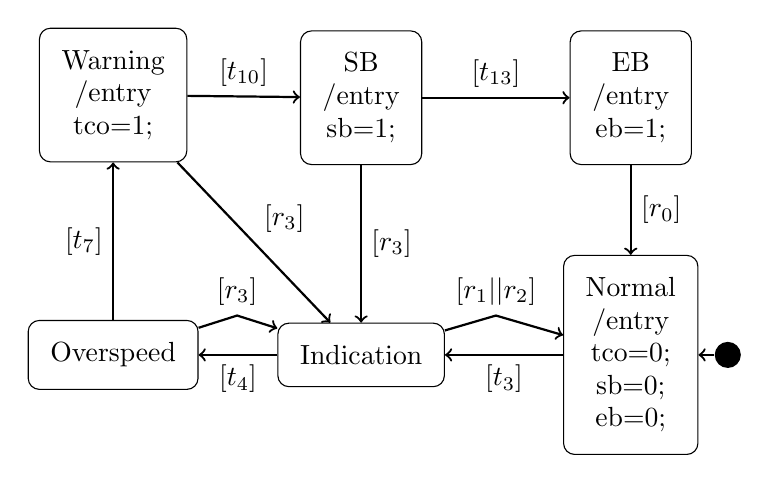
\begin{tikzpicture}
\node[initialstate] (initial) {};
\node[smstate,left=0.2cm of initial] (normal) {Normal\\/entry\\tco=0;\\sb=0;\\eb=0;};
\node[smstate,left=1.5cm of normal] (indication) {Indication};
\node[smstate,left= 1cm of indication] (overspeed) {Overspeed};
\node[smstate,above=2cm of overspeed] (warning) {Warning\\/entry\\tco=1;};
\node[smstate,above=2cm of indication] (sb) {SB\\/entry\\sb=1;};
\node[smstate] at(sb-|normal) (eb) {EB\\/entry\\eb=1;};

\draw[trans] (initial) -- (normal);
\draw[trans] (normal) --node[below] {$[t_3]$} (indication);
\draw[trans] (indication) -- node[below] {$[t_4]$}(overspeed);
\draw[trans] (overspeed) -- node[left] {$[t_7]$}(warning);
\draw[trans] (warning) -- node[above] {$[t_{10}]$}(sb);
\draw[trans] (sb) -- node[above] {$[t_{13}]$}(eb);
\draw[trans] (eb) -- node[right] {$[r_0]$}(normal);

\draw[trans] (indication) -- node[above,pos=1.0] {$[r_{1}||r_2]$} ($(indication)!0.5!(normal) + (0,0.5cm)$) -- (normal);
\draw[trans] (overspeed) -- node[above,pos=1.0] {$[r_3]$} ($(overspeed)!0.5!(indication) + (0,0.5cm)$) -- (indication);

\draw[trans] (warning) -- node[above right] {$[r_3]$}(indication);
\draw[trans] (sb) -- node[right] {$[r_3]$}(indication);
\end{tikzpicture}
}
\caption{State Machine of the TSM}
\label{fig:statemachine}
\end{figure}

\begin{figure*}[h]
\centering
\begin{tikzpicture}
\node[constraint] (c1) {$\lbrace t_{13} = v > (v_m + DV_\text{ebi}) \vee D_f > D_e\rbrace$};
\node[constraint, below=of c1] (c2) {$DV_\text{ebi} = 
   \left\{
   \begin{aligned}
   &7.5 & \IF v_m\leq 110\\
   &0.075 v_m-0.75 &\IF 110\le v_m \leq 210\\
   &15 & \IF 210 \leq v_m
   \end{aligned}
   \right. $
   };
\node[constraint, right=2 of c1] (c3) {$\lbrace D_\text{EBI} = D_e - T_\text{be} v \rbrace$};
\node[constraint, below=of c3] (c4) {$\lbrace D_\text{EBD} = D_t - s\rbrace $};


\node[parameter, left=1.5cm of c1, left= of c1] (df) {$D_\text{front}$};

\node[parameter, right=of c4] (dt) {$D_\text{target}$};
\node[parameter, below=0.5cm of dt] (s) {$s$};

\node[parameter, below=0.5cm of df] (vm) {$v_\text{mrsp}$};
\node[parameter, right=of c3] (tb) {$T_\text{be}$};
\node[parameter, above=0.4cm of tb] (ve) {$v_\text{est}$};

\draw[binding] (df) -- node[above] {$D_f$} (c1);
\draw[binding] (ve) -| node[near end, left] {$v$} (c1.50);
\draw[binding] (ve) -| node[near end, right] {$v$}(c3);
\draw[binding] (vm) -| node[near end, left] {$v_m$}(c1.200);
\draw[binding] (vm) -| node[near end, right] {$v_m$}(c2.150);
\draw[binding] (dt) -- node[above] {$D_t$} (c4);
\draw[binding] (s) -| node[near end, left] {$s$} (c4);
\draw[binding] (tb) -- node[above] {$T_\text{be}$}(c3);

\draw[double binding] (c1) -- node[right] {$DV_\text{ebi}$} ($(c2)!0.6!(c1)$) -| node [near end, right] {$DV_\text{ebi}$} (c2.21);
\draw[double binding] (c1) -- node[near start, above] {$D_\text{e}$} node [near end, below] {$D_\text{EBI} $}  (c3);
\draw[double binding] (c3) -- node[near start, right] {$D_\text{e}$} node [near end, left] {$D_\text{EBD}$} (c4);



\end{tikzpicture}
\caption{Parametric Diagram of the TSM}
\label{fig:parametric}
\end{figure*}



The approach described in the previous sections has been applied to the TSM function of the ETCS specification~\cite{ETCSSRS-Principles}. The specification describes the behavior in means of a transition table with the corresponding conditions for each transition. Such a specification can easily be modeled in terms of state machines and parametric diagrams: 
For every condition defined in the specification a Boolean variable $t_3,\ldots,t_{13},$ $r_0,\ldots,r_3$ was introduced, named according to the definitions  in~\cite{ETCSSRS-Principles}. The state machine can easily be deduced from the transition table using the introduced Boolean variables. The corresponding state machine of the TSM function is shown in Figure~\ref{fig:statemachine}. The concrete conditions are described and the introduced Boolean variables are bound by means of parametric diagrams. An excerpt of the parametric diagram of the TSM function is given in Figure~\ref{fig:parametric}. 

As a result, specifying the constraint blocks and creating the parametric diagram, as well as the state machine, was straightforward, where only the mathematical equations given in \cite{ETCSSRS-Principles} had to be translated to
constraint blocks and some notations had to be slightly modified to be parsed by our tools. Thus, the 
modeling effort for this example was very low and we assume that the modelling effort should scale very well
if other sub functions of this specification were modeled with the proposed approach.  

\paragraph{Model description}
In the TSM function state changes occur as soon as trigger conditions are fulfilled.
Under certain trigger conditions ($t_3$,$t_4$, \ldots) the system changes
its state machine state corresponding to different levels of intervention.
$t_3$ is a boolean expression that evaluates to true, if the current velocity
$V_\text{est}$ and the current train front position $D_\text{front}$ exceed the
line indicated by $D_I$ in Figure~\ref{fig:braking-curves}. Similarly,
$t_4,t_7,t_{10}$ and $t_{13}$ return true if and only if the train
exceeds $D_\text{P},D_\text{W},D_\text{SBI}$ or $D_\text{EBI}$ respectively.
When a new state machine state is entered, the \emph{entry}-actions write to the output
variables $\text{tco},\text{sb}$ and $\text{eb}$. These variables indicate the
activation of the traction cut-off, the service brake and the emergency brake.
The revocation conditions $r_0,\ldots,r_3$ describe the conditions
necessary for the intervention states to be revoked.

%figure for one column
%figure* for two column figures
\begin{figure}[b]
\centering
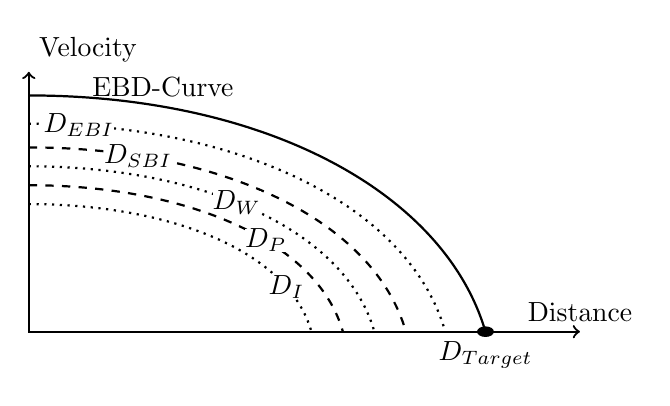
\begin{tikzpicture}[yscale=0.6]
% \draw[thick,red,xstep=1,ystep=1] (0,0) grid (8,6);
% \draw[very thin,red,xstep=0.1,ystep=0.1] (0,0) grid (8,6);
\draw[<->,thick] (0,5.5) node[above right] {Velocity} -- (0,0) -- (7,0) node[above] {Distance};
\node[below] (ebdfoot) at (5.8,0) {$D_\text{Target}$};
\draw[fill] (5.8,0) circle [radius=0.1];
\draw[thick] (0,5) to [out=0,in=100]  node[pos=0.2,above]{EBD-Curve} (5.8,0);
\node[below right] (ebifoot) at (5.2,0) {};
\draw[thick,dotted] (0,4.4) to [out=0,in=100] node[fill=white,inner sep=0,pos=0.08]{$D_\text{EBI}$} (ebifoot);
\node[below right] (sbifoot) at (4.7,0) {};
\draw[thick,dashed] (0,3.9) to [out=0,in=100] node[fill=white,inner sep=0,pos=0.2]{$D_\text{SBI}$} (sbifoot);
\node[below right] (wfoot) at (4.3,0) {};
\draw[thick,dotted] (0,3.5) to [out=0,in=100] node[fill=white,inner sep=0,pos=0.45]{$D_\text{W}$} (wfoot);
\node[below right] (pfoot) at (3.9,0) {};
\draw[thick,dashed] (0,3.1) to [out=0,in=100] node[fill=white,inner sep=0,pos=0.6]{$D_\text{P}$} (pfoot);
\node[below right] (ifoot) at (3.5,0) {};
\draw[thick,dotted] (0,2.7) to [out=0,in=100] node[fill=white,inner sep=0,pos=0.8]{$D_\text{I}$} (ifoot);
\end{tikzpicture}
\caption{Braking Curves of the TSM}
\label{fig:braking-curves}
\end{figure}   

The \emph{state invariants} of our test model are described by means of a parametric diagram and as an example in Figure~\ref{fig:parametric} the definition of trigger condition $t_{13}$ is shown. For convenience the definition of the other triggering conditions is omitted. 


All these triggering conditions depend on the train velocity and track relative
distance (position). The conditions can be calculated from the EBD
curve, compare Figure~\ref{fig:braking-curves}.
The EBD curve (emergency brake deceleration) maps the track relative distance to a
velocity, assuming a negative acceleration $A_\text{safe}$, such that zero speed is reached
at the target position ($D_\text{Target}$). The curve can be calculated by calculation of the 
braking distance $s$ as shown in Figure~\ref{fig:brakingdistance}.
The value of $A_\text{safe}$\footnote{For convenience we used a fixed value for
$A_\text{safe}$. According to the ETCS specification
\cite{ETCSSRS-Principles} up to seven values can be defined as a step function
dependent on the train speed.} is a conservative approximation that describes
the least deceleration that the emergency brakes of the train achieve when
fully activated.
Because the full activation of the emergency brakes needs some time, the curve
$D_\text{EBI}$ is shifted by a fixed time delay.
If the current distance-velocity-pair describing the train speed and position is
right or above this line, the emergency brakes are triggered.
In a similar way the other triggering conditions are defined by shifting the EBD
cure by fixed time delays.
   

The \emph{temporal evolution} of our test model is described by the parametric
diagram shown in Figure~\ref{fig:temporal-evolution}. The constraints in this diagram
restrict the time-continuous evolution of the trains front position and the velocity.
Therefore the acceleration $a$ of the train is restricted to values in the range $[-10,2]$. 
If the emergency brakes are activated (the train is in the state machine
state EB), the deceleration must be higher than prescribed by $A_\text{safe}$.  
As described in section~\ref{sec:concretization}, the discretized versions of
the constraints were used.

In total, our test model used for this evaluation contains 52 constraint properties,
including those shown in Figure~\ref{fig:brakingdistance},\ref{fig:temporal-evolution} and \ref{fig:parametric}.

\paragraph{Test case generation}

Table~\ref{tab:testgen} gives a summary of our test case generation. The test
case generation was performed on a system with 24 CPU cores running at 2.8 GHz
with 16 GB RAM. In the first step of our test case generation 50 abstract test
cases were calculated, which took less than a second. 
Then it took three and a half hours to generate the concrete test
cases from the 50 abstract test cases. The main reason, that this
computationally expensive task, is still applicable in acceptable time, is that
SMT instances for every test case can be solved in parallel. The test case
generation was run in parallel and on average 16.7 of the 24 CPUs were
utilized.

Given that the results from this TSM model can be generalized to hybrid systems
of comparable complexity, the runtime is acceptable. Yet, the
results indicate, that the utilization of a different computational backend,
e.g. analytical or numerical solvers, should be considered.

For every abstract test case a concrete
solution was calculated. Thus, our model abstraction seems appropriate. This might not always
be the case. If the test case generation of abstract test cases yields a low
percentage of solvable concrete test cases, this might be an indicator for
inappropriate abstraction or too restrictive constraints.


\begin{table}[h]
\centering
\begin{tabular}{|p{0.6\linewidth}|p{0.3\linewidth}|}
\hline
number of test cases generated & 50 \\
\hline
avg. test case length (test steps) & $2.84$ \\
 \hline
time for abstract test case generation & $0.8s$ \\
 \hline
time for calculation of concrete test cases & $3.5h$ \\
 \hline
 memory for test case generation & 8.4 GB\\
 \hline 
\end{tabular}
\caption{Results of the Test Case Generation for the TSM Model}
\label{tab:testgen}
\end{table}
\section{Conclusion}\label{sec:conc}
% ===========================================================================

 

In this technical report, 
a SysML model for the Ceiling Speed Monitor of the ETCS onboard controller 
has been presented and made publicly available on the website www.mbt-benchmarks.org, for the purpose 
of testing theory evaluation and MBT tool comparisons. 
The model has been represented in SysML, and a formal model semantics based on state transition systems has been specified by presenting the model's transition relation in propositional form.


A novel equivalence class testing strategy 
has been applied to derive tests from the CSM model in an automated way. This strategy allows 
test suite creation depending on a given fault model and guarantees completeness of the generated suites for all members of the associated fault domain. The evaluation shows that for certain types of mutants, the equivalence class testing strategy  is significantly stronger than that of other
test strategies, such as model transition coverage or MC/DC coverage.




\section{Ongoing and Future Work}\label{sec:futurework}
% ===========================================================================

The mutations used for the evaluation in this technical report were mainly constructed for illustration purposes.
Currently, we are evaluating the test strength of IECP test suites in comparison with  other model coverage criteria, using large numbers of mutants created by a random generator that mutates models and creates executable ``SUT'' code from each mutation.
These results will also be published on www.mbt-benchmarks.org.

The test suites described in this technical report focused on the active CSM only. We are currently working on a completion of the ETCS speed supervision functions, elaborating SysML sub-models for target speed monitoring and release speed monitoring. The resulting test suites will then also consider the switching between these three supervision functions.

The CSM test model inspires further investigations with respect to {\it product line testing}~\cite{DBLP:conf/icsoft/LamanchaUV09}: the system depends on a constant parameter $\sbz$ marking the
availability of a service brake to be used for intervention purposes in case of speed restriction violations (Section~\ref{sec:initialstate}). This parameter is not an input to the SUT, but to be kept  constant throughout a test suite, since it refers to the trains' hardware configurations. The SUT behaviour, however, 
depends on the value of  $\sbz$, so two different test suites have to be produced and exercised on the SUT, one for $\sbz = 0$, the other for $\sbz = 1$. This results in the challenge to identify in an automated way which test cases do not depend on $\sbz$, so that they have to be executed just once, and which cases have to be exercised for every possible value of $\sbz$.

\bibliographystyle{abbrv}
\bibliography{lit}

\end{document}
